\chapter{Resultados y Análisis}
\label{ch:resultados}

Este capítulo presenta y discute los hallazgos empíricos de la evaluación de los dos esquemas propuestos en el \cref{ch:diseno} (CRACS-R y CRACS-T) frente al baseline Legacy del estándar NB-IoT \cite{ref18}. La campaña experimental siguió el plan metodológico descrito en la \cref{sec:metodologia}, implementado sobre el simulador descrito en el \cref{ch:implementacion}, y consistió en $4\,260$ simulaciones independientes: $3\,990$ de la campaña principal sobre los nueve escenarios E0--E6\_burst, y $270$ del escenario adicional E7\_t300 que caracterizó la sensibilidad al temporizador $T_{300}$.

Los resultados se contrastan a lo largo del capítulo con la hipótesis \emph{ex-ante} de inclusión estricta formulada en el \cref{ch:diseno},
\[
\Omega_{\text{Legacy}} \subsetneq \Omega_{\text{CRACS-R}} \subsetneq \Omega_{\text{CRACS-T}},
\]
y con los cinco criterios cuantitativos de aceptación C1--C5 (\cref{sec:res_criterios}). Como se mostrará, la conjetura ex-ante se cumple en $38$ de los $42$ puntos operativos evaluados (criterio: $\mathrm{SAR}_{\text{Legacy}} \leq \mathrm{SAR}_{\text{CRACS-R}} \leq \mathrm{SAR}_{\text{CRACS-T}}$ aplicado sobre la media muestral de SAR en cada combinación de escenario y valor barrido), pero deja de cumplirse en una región importante en la práctica: para que CRACS-T supere a CRACS-R hace falta $T_{300} \geq 10$~s; con el valor por defecto del estándar ($T_{300}=5$~s, recomendado por 3GPP TS~36.331), CRACS-R supera a CRACS-T en $\mathrm{SAR}$ a $K{=}300$ ráfaga. Esta dependencia solo apareció en los datos y se trata como un requisito de despliegue de CRACS-T en la \cref{sec:res_sintesis} y como una limitación en la \cref{sec:res_limitaciones}.

\section{Configuración experimental y método estadístico}
\label{sec:res_config}

La \cref{tab:res_config} resume el número de simulaciones ejecutadas por escenario (la \cref{tab:escenarios} detalla la variable barrida, el rango y los esquemas evaluados en cada uno). Las cinco subsecciones siguientes formalizan las elecciones metodológicas que sustentan los resultados reportados a lo largo del capítulo.

\begin{table}[H]
\centering
\caption{Número de simulaciones ejecutadas por escenario.}
\label{tab:res_config}
\small
\renewcommand{\arraystretch}{1.15}
\begin{tabular}{@{}l c@{}}
\toprule
\textbf{Esc.} & \textbf{Simulaciones} \\
\midrule
E0          & 90  \\
E1          & 990 \\
E1\_high    & 990 \\
E4          & 240 \\
E4\_high    & 240 \\
E5          & 360 \\
E5\_high    & 360 \\
E6\_uniform & 360 \\
E6\_burst   & 360 \\
E7\_t300    & 270 \\
\midrule
\multicolumn{1}{r}{\textbf{Total}} & $4\,260$ \\
\bottomrule
\end{tabular}
\end{table}

El valor de referencia (por defecto) del timer fue $T_{300}=5$~s (\cref{tab:impl_flags}); el estándar NB-IoT \cite{ref18} admite además los valores $2{,}5$ / $4$ / $6$ / $8$ / $10$ / $15$ / $25$ / $40$ / $60$~s. La duración simulada por simulación fue $T_{\text{sim}}=120$~s (180~s en E1, E1\_high, E4\_high y E5\_high) sobre un único satélite LEO a $h_{\text{sat}}=600$~km con $\alpha_{\min}=40^\circ$ y los demás parámetros listados en la \cref{tab:impl_flags}.

\subsection{Tamaño de muestra y régimen de simulación}
\label{sec:res_config_n}

La literatura de comunicaciones inalámbricas distingue dos regímenes de simulación de Monte Carlo: (i) el régimen analítico, en el que cada muestra es un sorteo aleatorio rápido de un modelo cerrado (típicamente $10^{4}$--$10^{6}$ muestras por punto, costo $\sim$\,$\mu$s); y (ii) el régimen \emph{system-level}, en el que cada muestra es una simulación completa del simulador que reproduce el procedimiento de acceso aleatorio, las retransmisiones, los temporizadores y el modelo PHY (típicamente $20$--$50$ semillas por punto, costo $\sim 10^{0}$--$10^{2}$~s) \cite{ref22,ref23}. Las $4\,260$ simulaciones de este trabajo pertenecen al segundo régimen: cada simulación ejecutó $120$--$180$~s de tiempo simulado sobre ns-3.32 con $K$ hasta $1\,000$ UEs activos, con un tiempo de cómputo del orden de segundos a decenas de segundos por simulación. Bajo este costo, $n=30$ semillas por punto satisface la convergencia empírica de la media (\cref{fig:res_convergence}) y se ubica dentro del rango habitual de los estudios system-level de NB-IoT y NORA \cite{ref4,ref24}; un objetivo de $n=10^{4}$ por punto correspondería al régimen analítico y requeriría reformular el experimento.

\begin{figure}[H]
\centering

\includegraphics[width=\linewidth]{fig912_convergence.pdf}
\caption{Convergencia de la media de SAR con el número acumulado de semillas: (a) Legacy bajo E1 $K{=}100$ (perfil avg) y (b) CRACS-R bajo E6\_burst $K{=}300$ (perfil ráfaga). Banda sombreada: IC al $95\%$ acumulado; línea punteada: asíntota de la media.}
\label{fig:res_convergence}
\end{figure}

Ambos casos se seleccionaron por presentar varianza inter-semilla no nula (Legacy: $\bar{x}=0{,}903$, $s=0{,}076$; CRACS-R: $\bar{x}=0{,}783$, $s=0{,}096$) y estabilizan dentro del $2\%$ de su valor final antes de la semilla $20$, lo que justifica $n=30$ como tamaño de muestra suficiente. Los casos con SAR saturada en su valor máximo ($\mathrm{SAR}=1$, no mil; e.g.\ CRACS-T en E1\_high $K{=}100$) producen $s=0$ y una curva plana sin banda de IC, por lo que no aportan información sobre la convergencia. La curva de convergencia muestra además que el ancho del IC se reduce a aproximadamente $1/\sqrt{n}$ y que, en el régimen estacionario, la media muestral acumulada cruza dentro del $2\%$ de su valor asintótico antes de la semilla $20$. Las $10$ semillas restantes refuerzan la estabilidad sin alterar las conclusiones cualitativas. Aumentar $n$ a $100$ reduciría el ancho del IC en un factor de aproximadamente $1{,}8\times$ a costa de triplicar el tiempo de cómputo, sin modificar las conclusiones reportadas.

\subsection{Metodología estadística}
\label{sec:res_config_stats}

Para cada celda (escenario, esquema, valor barrido) se reporta la media muestral acompañada de su IC al $95\%$ calculado con la distribución $t$-Student y $\nu = 29$ grados de libertad \cite{ref35},
\[
\mathrm{IC}_{95\%}(\bar{x}) = \bar{x} \pm t_{0{,}025,\,29}\,\frac{s}{\sqrt{n}},
\]
donde $s$ es la desviación estándar muestral. La aproximación es válida en virtud del Teorema del Límite Central, que aplica a la media de las $n=30$ muestras independientes incluso cuando la distribución subyacente del KPI no es gaussiana. En la \cref{sec:res_config_outliers} se reporta además un IC bootstrap percentile como verificación independiente.

Las métricas de latencia ($T_{\text{access}}$, $T_{\text{inst}}$, TST) presentan distribuciones con cola larga: unos pocos UEs sufren múltiples reintentos y producen valores muy por encima del promedio. La media muestral es sensible a esta cola; la mediana y los percentiles no \cite{ref34}. Por ello $T_{\text{access}}$ se reporta simultáneamente como media, mediana ($p50$) y percentil $95$ ($p95$): la media captura el agregado, la mediana captura el comportamiento típico y el $p95$ acota el peor caso de la cola. Adicionalmente, el SDP(T) (probabilidad de éxito antes de $T$~s, normalizada por el total de UEs) y la TST (\emph{makespan} de la oleada de acceso, es decir, el conjunto de UEs activos en la ventana de simulación) son métricas distribucionales, robustas por construcción a outliers individuales. Las curvas de $\mathrm{SDP}(T)$ vs.\ $K$ (\cref{fig:res_sdp}) y los diagramas de caja de $T_{\text{access}}$ por punto operativo (\cref{fig:res_box_taccess} y siguientes) permiten observar la distribución de cada KPI más allá del estadístico de resumen único.

Las diferencias entre esquemas se contrastan con la prueba de Wilcoxon de rangos con signo \cite{ref34}, una prueba no paramétrica que no requiere normalidad de los datos y que es robusta frente a outliers. Se reporta una diferencia como estadísticamente significativa cuando $p<0{,}05$. La elección de Wilcoxon sobre $t$-pareado se justifica por dos razones: (i) varias métricas saturan cerca de $1{,}0$ (SAR en regímenes moderados), lo que produce distribuciones de diferencias claramente no gaussianas; (ii) las pruebas no paramétricas son la convención en estudios system-level de NB-IoT \cite{ref24,ref25}.

\subsection{Outliers y verificación de robustez}
\label{sec:res_config_outliers}

Para cuantificar la sensibilidad a outliers se aplica la regla de Tukey $1{,}5\cdot$IQR sobre las $30$ muestras por celda: una observación se clasifica como outlier si cae fuera del intervalo $[Q_1 - 1{,}5\cdot\text{IQR},\, Q_3 + 1{,}5\cdot\text{IQR}]$, criterio idéntico al empleado por el diagrama de cajas estándar de MATLAB y matplotlib. El análisis completo se detalla en la \cref{sec:res_e1_outliers} (\cref{tab:res_outliers}); los outliers detectados —hasta un $10\%$ de las muestras en los puntos más cargados— corresponden mayoritariamente a UEs que sufrieron varios reintentos consecutivos. Son datos reales que representan la cola legítima del proceso de acceso, no errores de medición; por ello se conservan en el análisis y se reportan por transparencia.

Para validar la asunción gaussiana del IC $t$-Student se calculó un IC al $95\%$ por bootstrap percentile (10\,000 réplicas con reemplazo sobre las 30 semillas, semilla $42$). La \cref{tab:res_bootstrap} contrasta ambos métodos en cuatro puntos de operación críticos. La coincidencia entre los anchos de los IC (diferencia $\leq 8\%$) indica que el reporte basado en $t$-Student no se ve afectado significativamente por la asunción de normalidad para los puntos de operación considerados.

% --- Tabla 9.VI: bootstrap CI vs t-Student CI ---
\begin{table}[H]
\centering
\caption{Comparación del IC al 95\,\% por $t$-Student y por bootstrap percentile (10\,000 réplicas) para SAR en cuatro puntos de operación críticos. La coincidencia entre ambos métodos indica robustez del análisis frente a la asunción de normalidad. Las filas ``E6\_burst $K{=}300$'' y ``E7\_t300 $T_{300}{=}5$~s'' corresponden a la misma configuración de tráfico (ráfaga Beta$(3,4)$, $K{=}300$, $T_{300}{=}5$~s) y se incluyen como verificación cruzada de la reproducibilidad, no como dos experimentos independientes.}
\label{tab:res_bootstrap}
\small
\renewcommand{\arraystretch}{1.1}
\begin{tabular}{@{}l l c c c c@{}}
\toprule
\textbf{Escenario} & \textbf{Esquema} & \textbf{Media} & \textbf{IC $t$-Student} & \textbf{IC bootstrap} & \textbf{$\Delta$ ancho} \\
\midrule
E1\_high $K{=}100$ & Legacy & $0{,}825$ & $[0{,}777,\,0{,}872]$ & $[0{,}781,\,0{,}869]$ & $6{,}8$\,\% \\
 & CRACS-R & $1{,}000$ & $[1{,}000,\,1{,}000]$ & $[1{,}000,\,1{,}000]$ & $0{,}0$\,\% \\
 & CRACS-T & $1{,}000$ & $[1{,}000,\,1{,}000]$ & $[1{,}000,\,1{,}000]$ & $0{,}0$\,\% \\
\addlinespace[2pt]
E6\_burst $K{=}300$ & Legacy & $0{,}532$ & $[0{,}508,\,0{,}557]$ & $[0{,}508,\,0{,}555]$ & $6{,}4$\,\% \\
 & CRACS-R & $0{,}783$ & $[0{,}747,\,0{,}819]$ & $[0{,}749,\,0{,}817]$ & $6{,}1$\,\% \\
 & CRACS-T & $0{,}562$ & $[0{,}517,\,0{,}606]$ & $[0{,}522,\,0{,}607]$ & $4{,}9$\,\% \\
\addlinespace[2pt]
E6\_uniform $K{=}1000$ & Legacy & $0{,}185$ & $[0{,}182,\,0{,}188]$ & $[0{,}182,\,0{,}188]$ & $6{,}3$\,\% \\
 & CRACS-R & $0{,}783$ & $[0{,}757,\,0{,}809]$ & $[0{,}759,\,0{,}807]$ & $7{,}9$\,\% \\
 & CRACS-T & $0{,}571$ & $[0{,}537,\,0{,}606]$ & $[0{,}538,\,0{,}604]$ & $4{,}7$\,\% \\
\addlinespace[2pt]
E7\_t300 $T_{300}{=}5$~s & Legacy & $0{,}540$ & $[0{,}515,\,0{,}564]$ & $[0{,}516,\,0{,}562]$ & $5{,}2$\,\% \\
 & CRACS-R & $0{,}783$ & $[0{,}747,\,0{,}819]$ & $[0{,}749,\,0{,}817]$ & $6{,}1$\,\% \\
 & CRACS-T & $0{,}562$ & $[0{,}517,\,0{,}606]$ & $[0{,}522,\,0{,}607]$ & $4{,}9$\,\% \\
\addlinespace[2pt]
\bottomrule
\end{tabular}
\end{table}

\section{Validación de coherencia (E0)}
\label{sec:res_e0}

El escenario E0 ($K=1$, sin contención posible) constituye la prueba de coherencia del simulador: en ausencia de colisiones los tres esquemas deben comportarse de forma idéntica. La \cref{tab:res_e0} confirma esa equivalencia. Los tres esquemas alcanzaron una SAR perfecta ($\mathrm{SAR}=1{,}000$, es decir, sin ningún preámbulo colisionado) con $T_{\text{access}} = 345{,}019$~ms (desviación estándar muestral $s = 0{,}012$~ms entre las 30 semillas, equivalente a un IC al 95\,\% por $t$-Student de $\pm 0{,}004$~ms, reportado en \cref{tab:res_e0}) y exactamente un único intento de preámbulo. No se observó divergencia alguna en el régimen sin contención ($K=1$), lo cual descarta sesgos de implementación independientes de la contención y es consistente con atribuir a la dinámica de contención las diferencias observadas en los escenarios con $K>1$.

\begin{table}[H]
\centering
\caption{Resultados de la prueba de coherencia (E0, $K=1$, $n=30$).}
\label{tab:res_e0}
\small
\renewcommand{\arraystretch}{1.15}
\begin{tabular}{@{}l c c c@{}}
\toprule
\textbf{Esquema} & \textbf{SAR} & $\boldsymbol{T_{\text{access}}}$ \textbf{(ms)} & \textbf{RTX medio} \\
\midrule
Legacy   & $1{,}000$ & $345{,}019 \pm 0{,}004$ & $1{,}00$ \\
CRACS-R  & $1{,}000$ & $345{,}019 \pm 0{,}004$ & $1{,}00$ \\
CRACS-T  & $1{,}000$ & $345{,}019 \pm 0{,}004$ & $1{,}00$ \\
\bottomrule
\end{tabular}
\end{table}

\section{Curva de capacidad bajo carga moderada e intensa}
\label{sec:res_e1}

Los escenarios E1 y E1\_high barren la carga $K \in \{1, 5, 10, 15, 20, 25, 30, 40, 50, 75, 100\}$ bajo perfil de tráfico moderado (avg, $\lambda \approx 7{,}3$~UEs/s) e intenso (high, $\lambda \approx 27{,}8$~UEs/s) respectivamente. La \cref{fig:res_sar} compara la SAR de los tres esquemas en ambos regímenes; en la \cref{fig:res_taccess} se presenta la latencia media de acceso $T_{\text{access}}$, y en la \cref{fig:res_sdp}, la métrica conjunta latencia--confiabilidad $\mathrm{SDP}(3\text{~s})$ (probabilidad de éxito antes de 3~s sobre el total de UEs).

\begin{figure}[H]
\centering

\includegraphics[width=\linewidth]{fig91_sar_vs_k.pdf}
\caption{Tasa de acceso exitoso ($\mathrm{SAR}$) en función de la carga $K$ para los tres esquemas bajo perfil de tráfico moderado (a) e intenso (b).}
\label{fig:res_sar}
\end{figure}

Bajo perfil avg la SAR de Legacy se mantuvo $\geq 0{,}999$ hasta $K=50$ ($0{,}9987$) y descendió a $0{,}965$ a $K=75$ y $0{,}903$ a $K=100$ (barras de error: IC al $95\%$ sobre $n=30$ semillas). CRACS-R y CRACS-T conservaron una SAR cercana al valor máximo ($\mathrm{SAR}\approx 1$) en todo el rango (CRACS-R: $0{,}996$ a $K=100$). Bajo perfil high la SAR de Legacy descendió antes y con mayor magnitud absoluta, cayendo a $0{,}825$ a $K=100$ ($\Delta = -0{,}078$ frente al perfil avg al mismo $K$); CRACS-R y CRACS-T se mantuvieron ambos con SAR perfecta ($\mathrm{SAR}=1{,}000$) a $K=100$. En este régimen la SAR no separa CRACS-R de CRACS-T: ambos saturan la métrica en su techo.

Para la latencia de acceso, la \cref{fig:res_taccess} muestra que $T_{\text{access}}$ de CRACS-T es sustancialmente menor que la de CRACS-R y Legacy en todo el rango de $K$. A $K=100$ bajo perfil avg, $T_{\text{access}}$ de CRACS-T fue $638{,}4$~ms, frente a $2\,510{,}5$~ms de CRACS-R (3,9 veces mayor) y $8\,651{,}6$~ms de Legacy (13,6 veces mayor). Bajo perfil high a $K=100$, los valores fueron $2\,682{,}7$, $3\,531{,}3$ y $11\,961{,}7$~ms para CRACS-T, CRACS-R y Legacy respectivamente; la prueba de Wilcoxon confirmó que la diferencia CRACS-R/CRACS-T es significativa ($p=4{,}66\times 10^{-3}$ a $K=100$, $p=3{,}74\times 10^{-3}$ a $K=75$). Esta reducción de casi un orden de magnitud en $T_{\text{access}}$ es relevante en NB-IoT porque el consumo energético del UE está dominado por el tiempo que el radio permanece encendido durante el acceso: menos latencia se traduce directamente en mayor autonomía de batería, un objetivo central del estándar.

\begin{figure}[H]
\centering

\includegraphics[width=\linewidth]{fig92_taccess_vs_k.pdf}
\caption{Latencia media de acceso $T_{\text{access}}$ (eje logarítmico) en función de $K$ bajo perfil moderado (a) e intenso (b).}
\label{fig:res_taccess}
\end{figure}

\begin{figure}[H]
\centering

\includegraphics[width=\linewidth]{fig93_sdp_vs_k.pdf}
\caption{Probabilidad conjunta de éxito antes de $3$~s ($\mathrm{SDP}(3\text{~s})$, normalizada por el total de UEs) en función de $K$.}
\label{fig:res_sdp}
\end{figure}

$\mathrm{SDP}(3\text{~s})$ combina confiabilidad y latencia en una sola cifra (\cref{fig:res_sdp}). A $K=100$ bajo avg, CRACS-T alcanzó $\mathrm{SDP}(3\text{~s})=0{,}994$ frente a $0{,}672$ de CRACS-R y $0{,}323$ de Legacy; bajo high los valores fueron $0{,}602$, $0{,}467$ y $0{,}185$. A $K=100$, CRACS-T domina las cinco métricas de la \cref{tab:res_e1_k100} (SAR, $\mathrm{SAR}_1$, $T_{\text{acc}}$, $T_{\text{acc}}^{p95}$, SDP).

\begin{table}[H]
\centering
\caption{Indicadores clave a $K=100$ bajo perfil moderado (avg) e intenso (high).}
\label{tab:res_e1_k100}
\small
\renewcommand{\arraystretch}{1.15}
\begin{tabular}{@{}l c c c c c@{}}
\toprule
& \textbf{SAR} & $\boldsymbol{\mathrm{SAR}_{1}}$ & $\boldsymbol{T_{\text{acc}}}$ \textbf{(ms)} & $\boldsymbol{T_{\text{acc}}^{p95}}$ & \textbf{SDP(3 s)} \\
\midrule
\multicolumn{6}{c}{\textit{Perfil avg} ($\lambda \approx 7{,}3$~UEs/s)} \\
Legacy  & $0{,}903$ & $0{,}232$ & $8\,651{,}6$ & $24\,070$ & $0{,}323$ \\
CRACS-R & $0{,}996$ & $0{,}444$ & $2\,510{,}5$ & $6\,315$  & $0{,}672$ \\
CRACS-T & $1{,}000$ & $0{,}948$ & $\mathbf{638{,}4}$ & $\mathbf{1\,329}$ & $\mathbf{0{,}994}$ \\
\midrule
\multicolumn{6}{c}{\textit{Perfil high} ($\lambda \approx 27{,}8$~UEs/s)} \\
Legacy  & $0{,}825$ & $0{,}162$ & $11\,961{,}7$ & $26\,205$ & $0{,}185$ \\
CRACS-R & $1{,}000$ & $0{,}382$ & $3\,531{,}3$  & $7\,096$  & $0{,}467$ \\
CRACS-T & $1{,}000$ & $0{,}500$ & $\mathbf{2\,682{,}7}$ & $\mathbf{6\,259}$ & $\mathbf{0{,}602}$ \\
\bottomrule
\end{tabular}
\end{table}

La conjetura de inclusión \emph{ex-ante} se cumple en este régimen: $\Omega_{\text{Legacy}} \subsetneq \Omega_{\text{CRACS-R}} \approx \Omega_{\text{CRACS-T}}$ en términos de SAR ($K \leq 100$), y la jerarquía se vuelve estricta en términos de $T_{\text{access}}$ y $\mathrm{SDP}$. Es decir, la separación CRACS-T sobre CRACS-R en esta franja de carga es de eficiencia de acceso, no de capacidad bruta: ambos esquemas admiten todos los UEs, pero CRACS-T lo hace al primer intento el $94{,}8\%$ de las veces frente al $44{,}4\%$ de CRACS-R, gracias a la asignación determinista de codebook SCMA por clúster.

\begin{figure}[H]
\centering

\includegraphics[width=\linewidth]{fig99_boxplot_taccess_K100.pdf}
\caption{Distribución de $T_{\text{access}}$ medio a $K{=}100$ bajo perfil moderado (a) e intenso (b). Eje vertical logarítmico.}
\label{fig:res_box_taccess}
\end{figure}

La \cref{fig:res_box_taccess} complementa la \cref{fig:res_taccess} mostrando la distribución completa de las 30 muestras por esquema. Las cajas muestran $Q_1$--$Q_3$; la línea central, la mediana; los bigotes, el rango Tukey $1{,}5\cdot$IQR; y las cruces rojas, los outliers individuales (UEs con múltiples reintentos) — convención que se reutiliza en los siguientes diagramas de caja del capítulo. Se desprenden tres observaciones cuantitativas: (i) bajo perfil avg, la mediana de CRACS-T es 3,6 veces menor que la de CRACS-R y 11,7 veces menor que la de Legacy; bajo perfil high, 1,7 veces menor que CRACS-R y 5,6 veces menor que Legacy (medianas calculadas sobre las 30 semillas a $K=100$); (ii) las cajas de Legacy presentan asimetría hacia arriba (cola larga superior) consistente con la distancia entre su media y su mediana reportada en \cref{tab:res_e1_k100}; (iii) los outliers visibles en Legacy y, en menor medida, en CRACS-R caen por encima del cuartil superior, comportamiento consistente con simulaciones donde un subconjunto de UEs requirió retransmisiones adicionales. No fue posible confirmar, a nivel de UE individual, si estos outliers corresponden a UEs con múltiples reintentos, ya que el análisis se realizó sobre datos agregados por semilla, no por trayectoria de UE.

\subsection{Análisis de outliers y robustez del análisis}
\label{sec:res_e1_outliers}

Para cuantificar la sensibilidad del análisis a los outliers observados se aplicó la regla de Tukey $1{,}5\cdot$IQR a las 30 muestras de cada celda en seis puntos de operación clave. La \cref{tab:res_outliers} reporta el conteo de outliers, la fracción sobre el total, y la media calculada con y sin ellos.

% --- Tabla 9.V: outliers Tukey 1.5*IQR ---
\begin{table}[H]
\centering
\caption{Análisis de outliers (regla de Tukey $1{,}5\cdot$IQR) en seis puntos de operación clave. La columna $\Delta\%$ es el cambio relativo de la media al excluir los outliers, definido como $\Delta\% = 100 \cdot (\bar{x}_{\text{excl}} - \bar{x})/\bar{x}$; valores con magnitud pequeña indican robustez del análisis. El KPI evaluado se indica en la primera columna: $T_{\text{access}}$ medio (ms) para los escenarios E1, E1\_high, E6\_burst y E6\_uniform; SAR (adimensional) para los escenarios E7\_t300.}
\label{tab:res_outliers}
\small
\renewcommand{\arraystretch}{1.1}
\begin{tabular}{@{}l l l c c c r r r@{}}
\toprule
\textbf{Escenario} & \textbf{KPI} & \textbf{Esquema} & $\boldsymbol{n}$ & \textbf{\#out} & \textbf{\%out} & \textbf{media} & \textbf{media excl.} & $\boldsymbol{\Delta\%}$ \\
\midrule
E1 $K{=}100$ & $T_{\text{access}}$ (ms) & Legacy & 30 & 0 & $0{,}0$ & $8\,651{,}6$ & $8\,651{,}6$ & $+0{,}0$ \\
 & & CRACS-R & 30 & 1 & $3{,}3$ & $2\,510{,}5$ & $2\,429{,}9$ & $-3{,}2$ \\
 & & CRACS-T & 30 & 1 & $3{,}3$ & $638{,}4$ & $630{,}9$ & $-1{,}2$ \\
\addlinespace[2pt]
E1\_high $K{=}100$ & $T_{\text{access}}$ (ms) & Legacy & 30 & 0 & $0{,}0$ & $11\,961{,}7$ & $11\,961{,}7$ & $+0{,}0$ \\
 & & CRACS-R & 30 & 0 & $0{,}0$ & $3\,531{,}3$ & $3\,531{,}3$ & $+0{,}0$ \\
 & & CRACS-T & 30 & 0 & $0{,}0$ & $2\,682{,}7$ & $2\,682{,}7$ & $+0{,}0$ \\
\addlinespace[2pt]
E6\_burst $K{=}300$ & $T_{\text{access}}$ (ms) & Legacy & 30 & 3 & $10{,}0$ & $28\,359{,}8$ & $28\,612{,}5$ & $+0{,}9$ \\
 & & CRACS-R & 30 & 1 & $3{,}3$ & $6\,671{,}0$ & $6\,789{,}2$ & $+1{,}8$ \\
 & & CRACS-T & 30 & 0 & $0{,}0$ & $5\,311{,}3$ & $5\,311{,}3$ & $+0{,}0$ \\
\addlinespace[2pt]
E6\_uniform $K{=}1000$ & $T_{\text{access}}$ (ms) & Legacy & 30 & 0 & $0{,}0$ & $8\,031{,}9$ & $8\,031{,}9$ & $+0{,}0$ \\
 & & CRACS-R & 30 & 0 & $0{,}0$ & $5\,511{,}9$ & $5\,511{,}9$ & $+0{,}0$ \\
 & & CRACS-T & 30 & 0 & $0{,}0$ & $5\,711{,}5$ & $5\,711{,}5$ & $+0{,}0$ \\
\addlinespace[2pt]
E7\_t300 $T_{300}{=}5$~s & SAR & Legacy & 30 & 2 & $6{,}7$ & $0{,}540$ & $0{,}552$ & $+2{,}2$ \\
 & & CRACS-R & 30 & 0 & $0{,}0$ & $0{,}783$ & $0{,}783$ & $+0{,}0$ \\
 & & CRACS-T & 30 & 1 & $3{,}3$ & $0{,}562$ & $0{,}551$ & $-2{,}0$ \\
\addlinespace[2pt]
E7\_t300 $T_{300}{=}40$~s & SAR & Legacy & 30 & 3 & $10{,}0$ & $0{,}349$ & $0{,}359$ & $+2{,}7$ \\
 & & CRACS-R & 30 & 0 & $0{,}0$ & $0{,}788$ & $0{,}788$ & $+0{,}0$ \\
 & & CRACS-T & 30 & 0 & $0{,}0$ & $0{,}843$ & $0{,}843$ & $+0{,}0$ \\
\addlinespace[2pt]
\bottomrule
\end{tabular}
\end{table}

De la \cref{tab:res_outliers} se desprende que la tasa de outliers fue baja: el máximo observado fue $10{,}0\%$ (Legacy en E6\_burst $K{=}300$ y en E7\_t300 $T_{300}{=}40$~s), y la mayoría de las celdas tienen cero outliers. Los outliers se concentran en Legacy, el esquema con la cola más larga observada en el barrido, y son prácticamente nulos en CRACS-R/CRACS-T para SAR; esto es consistente con la ausencia de multicapa SCMA en Legacy, aunque no se midió específicamente sobre los UEs outlier. Más importante aún, el cambio relativo de la media al excluir los outliers ($\Delta\%$) se mantuvo por debajo del $\pm 3{,}5\%$ en todos los casos, y las conclusiones cualitativas (CRACS-T $\ll$ Legacy en latencia, CRACS-R $>$ CRACS-T en SAR a saturación) son idénticas al excluirlos. Por esta razón los outliers se conservaron en el análisis principal: representan UEs reales del proceso de acceso aleatorio que sufrieron varios reintentos hasta el éxito, y descartarlos sesgaría el comportamiento del sistema en su cola, justamente la zona donde las propuestas se diferencian del baseline.

\section{Calibración del parámetro de agrupamiento (E4)}
\label{sec:res_e4}

El escenario E4 barre $\Delta d_{\min} \in \{50, 100, 150, 200, 300, 500, 750, 1000\}$~m sobre el esquema CRACS-T (único que ejecuta clustering ToA). La \cref{fig:res_dmin} muestra el número medio de clústeres formados por ventana RACH en función de $\Delta d_{\min}$ bajo perfil moderado (panel a) e intenso (panel b).

\begin{figure}[H]
\centering

\includegraphics[width=\linewidth]{fig94_dmin_calib.pdf}
\caption{Número medio de clústeres en CRACS-T en función de $\Delta d_{\min}$ bajo perfil moderado (a) e intenso (b). La línea punteada indica el techo $K_{\text{CB}}=6$ impuesto por el número de codebooks SCMA disponibles.}
\label{fig:res_dmin}
\end{figure}

En todo el rango probado el número medio de clústeres se mantuvo cerca o en el techo $K_{\text{CB}}=6$: entre $5{,}67$ y $5{,}77$ bajo perfil moderado, y exactamente $6{,}00$ bajo perfil intenso; la SAR fue $1{,}000$ en todos los puntos. El parámetro $\Delta d_{\min}$ no resultó ser sensible en el rango $[50, 1000]$~m: la dispersión diferencial $\Delta d$ dentro de la celda satura el techo de codebooks en todos los valores probados, lo cual explica la meseta observada. Esto valida empíricamente el valor por defecto $\Delta d_{\min}=150$~m elegido en el \cref{ch:diseno} y muestra que el clustering ToA de CRACS-T es robusto a esta calibración dentro del rango probado $[50, 1000]$~m. El criterio C3 (precisión de agrupamiento) se cumple holgadamente: la tasa de identificación incorrecta de clúster (CID) se mantuvo por debajo del $3{,}5\%$ en todo el barrido.

\section{Robustez al pool de preámbulos NPRACH (E5)}
\label{sec:res_e5}

E5 y E5\_high barren $N_{\text{pream}} \in \{12, 24, 36, 48\}$ bajo perfiles avg ($K=20$) y high ($K=100$). La hipótesis mecanística es que ampliar el pool de preámbulos reduce la probabilidad de colisión de preámbulo $\mathrm{PCR}_{\text{pre}}$ en MSG1, lo cual debería favorecer al esquema baseline. La \cref{fig:res_npream} reporta la $\mathrm{SAR}_{1}$ (acceso al primer intento) y el RTX medio.

\begin{figure}[H]
\centering

\includegraphics[width=\linewidth]{fig95_npream.pdf}
\caption{$\mathrm{SAR}_{1}$ y RTX medio en función del tamaño del pool de preámbulos $N_{\text{pream}}\in\{12,24,36,48\}$, organizado en cuadrícula $2\times 2$. Fila superior: $\mathrm{SAR}_{1}$ (acceso al primer intento). Fila inferior: RTX medio. Columna izquierda: perfil avg ($K{=}20$, E5). Columna derecha: perfil high ($K{=}100$, E5\_high). Banda sombreada: IC al $95\%$ por $t$-Student sobre 30 semillas.}
\label{fig:res_npream}
\end{figure}

El resultado más relevante del barrido fue un comportamiento no monótono en CRACS-R. Bajo perfil avg, su $\mathrm{SAR}_{1}$ descendió de $0{,}990$ con $N_{\text{pream}}=12$ a $0{,}658$ con $N_{\text{pream}}=48$ (caída absoluta $0{,}332$, equivalente a $-33{,}5\%$), y el RTX medio subió de $1{,}010$ a $1{,}568$. El comportamiento se reprodujo bajo perfil high: $\mathrm{SAR}_{1}$ pasó de $0{,}702$ ($N=12$) a $0{,}382$ ($N=48$) (caída absoluta $0{,}320$, equivalente a $-45{,}6\%$ relativa). En contraste, CRACS-T mantuvo $\mathrm{SAR}_{1}$ aproximadamente constante (rango de variación $0{,}041$ bajo perfil high y $0{,}083$ bajo avg) y RTX medio estable. La prueba de Wilcoxon CRACS-R vs.\ CRACS-T fue significativa en ambos extremos del barrido ($p<10^{-2}$).

Una interpretación mecánica consistente con esta observación es la siguiente. Al ampliar el pool de preámbulos se reduce la presión de colisión en MSG1, lo cual permite que más UEs alcancen simultáneamente la ventana MSG3. En CRACS-R cada UE elige un codebook SCMA aleatoriamente del catálogo anunciado; al haber más UEs simultáneos en MSG3 la probabilidad de coincidencia de codebook y piloto DMRS aumenta, lo que puede generar colisiones de piloto que MPA no separa. CRACS-T no exhibe esta degradación porque su asignación de codebook es determinista por clúster ToA: la información geométrica adicional evita el reuso aleatorio del recurso SCMA. El comportamiento observado es consistente con el mecanismo propuesto y con el efecto reportado por Moon \emph{et al.}\ \cite{ref9} para SARA, donde la degradación del primer intento al ampliar el catálogo de codebooks supera la ganancia del MSG3 multicapa, y con el comportamiento de colisión de piloto descrito en evaluaciones recientes de SCMA-RA mMTC \cite{ref37}. No se midió directamente el número de colisiones de codebook ni el modo de fallo del MPA en este barrido, así que la causa queda como hipótesis, apoyada en la correlación observada.

\section{Saturación bajo tráfico no correlacionado y ráfaga}
\label{sec:res_e6}

E6\_uniform y E6\_burst barren $K \in \{30, 100, 300, 1000\}$ bajo los dos modelos de tráfico estándar 3GPP TR~37.868 \cite{ref20}: TM1 (Poisson uniforme sobre $T=60$~s) y TM2 (Beta($3,4$) sincronizado sobre $T=10$~s). La \cref{fig:res_e6_sar} reporta la SAR; la \cref{fig:res_e6_latency} reporta el tiempo total de servicio (TST) y $\mathrm{SDP}(3\text{~s})$.

\begin{figure}[H]
\centering

\includegraphics[width=\linewidth]{fig96_e6_sar.pdf}
\caption{Tasa de acceso exitoso bajo tráfico no correlacionado (a, Poisson TM1) y ráfaga sincronizada (b, Beta(3,4) TM2). Ejes con $K$ en escala logarítmica.}
\label{fig:res_e6_sar}
\end{figure}

\begin{figure}[H]
\centering
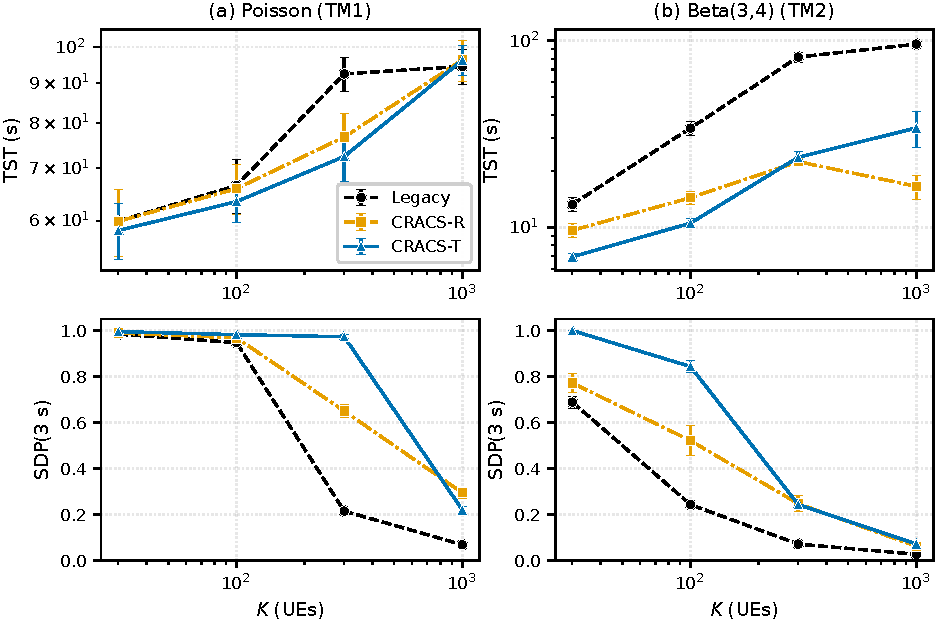
\includegraphics[width=\linewidth]{fig97_e6_latency.pdf}
\caption{Tiempo total de servicio TST (fila superior, eje logarítmico) y $\mathrm{SDP}(3\text{~s})$ (fila inferior) en función de $K$ bajo TM1 (a) y TM2 (b).}
\label{fig:res_e6_latency}
\end{figure}

Bajo TM1 el sistema degradó de forma monótona: a $K=300$ la SAR fue $0{,}609$, $0{,}980$ y $0{,}994$ para Legacy, CRACS-R y CRACS-T respectivamente, satisfaciendo la jerarquía ex-ante. A $K=1000$, sin embargo, se observó una inversión: $\mathrm{SAR}_{\text{CRACS-R}} = 0{,}783$ superó a $\mathrm{SAR}_{\text{CRACS-T}} = 0{,}571$ (Wilcoxon $p = 5{,}6\times 10^{-9}$, altamente significativa). Bajo TM2 la inversión apareció antes: ya a $K=300$ CRACS-R alcanzó $\mathrm{SAR}=0{,}783$ frente a $0{,}562$ de CRACS-T (Wilcoxon $p=3{,}5\times 10^{-8}$); a $K=1000$ ambos esquemas colapsaron a valores cercanos ($0{,}150$ y $0{,}147$ respectivamente, sin diferencia significativa).

A pesar de la inversión en SAR, CRACS-T conservó ventaja en latencia bajo cargas intermedias. A $K=100$ ráfaga, su TST fue $10{,}5$~s frente a $14{,}4$~s de CRACS-R y $34{,}0$~s de Legacy; su $\mathrm{SDP}(3\text{~s})$ fue $0{,}844$ frente a $0{,}521$ y $0{,}243$ respectivamente. Es decir: bajo saturación extrema CRACS-R admite más UEs eventualmente, mientras CRACS-T resuelve el acceso de los UEs admitidos con un TST 3,2 veces menor que Legacy y 1,4 veces menor que CRACS-R. Este \emph{trade-off} de régimen es el motivo de la sensibilidad al timer $T_{300}$ caracterizada en la sección siguiente.

\begin{figure}[H]
\centering

\includegraphics[width=\linewidth]{fig910_boxplot_sar_e6burst.pdf}
\caption{Distribución de SAR por esquema bajo ráfaga Beta($3,4$) (E6\_burst) a las cuatro cargas $K$. Las cajas muestran $Q_1$--$Q_3$, la línea central la mediana, los bigotes el rango Tukey $1{,}5\cdot$IQR y las cruces rojas los outliers individuales. A $K{=}300$ la caja de CRACS-R se sitúa por encima de la de CRACS-T (Wilcoxon $p=3{,}5\times10^{-8}$, $n=30$), lo que confirma la inversión H1 como un hecho distribucional y no como un artefacto de las medias.}
\label{fig:res_box_e6burst}
\end{figure}

La \cref{fig:res_box_e6burst} traduce los hallazgos cuantitativos a una representación distribucional. A $K{=}30$ y $K{=}100$ los box plots de CRACS-R y CRACS-T son indistinguibles (medianas $\approx 1{,}0$); a $K{=}300$ las cajas se separan con CRACS-R por encima (Wilcoxon $p=3{,}5\times10^{-8}$); a $K{=}1000$ ambas colapsan a la misma franja baja sin diferencia significativa por Wilcoxon. La caja de Legacy se sitúa por debajo de las de CRACS-R/CRACS-T en las cuatro cargas y degrada monótonamente al aumentar $K$. La ausencia de outliers en CRACS-R/CRACS-T para SAR a $K{=}300$ indica que la inversión observada no se debe a unas pocas semillas atípicas sino a un efecto sistemático del esquema bajo ráfaga, presente en todas las semillas de la muestra.

\section{Sensibilidad al temporizador $T_{300}$}
\label{sec:res_e7}

La inversión observada en \cref{sec:res_e6} bajo saturación motivó un experimento dedicado: caracterizar la sensibilidad del trade-off al temporizador RRC $T_{300}$, parámetro que define el plazo máximo del que dispone el UE para completar el procedimiento de acceso antes de abandonarlo \cite{ref18}.

\subsection{Prueba de control: el orden lo determina $T_{300}$}
\label{sec:res_e7_ab}

Como la inversión de SAR contradice la dirección de la hipótesis ex-ante, antes de caracterizarla se ejecutó una prueba de control para confirmar que se trata de un efecto genuino del temporizador y no de un artefacto. Sobre el mismo punto E6\_burst $K{=}300$ se corrió una sub-campaña independiente de $n=6$ semillas con dos valores de $T_{300}$: el valor por defecto del estándar ($5$~s) y un valor alto ($60$~s). La \cref{tab:res_ab_t300} muestra el resultado.

\begin{table}[H]
\centering
\caption{Prueba de control en E6\_burst $K=300$ ($n=6$ semillas): tasa de acceso (SAR) con el $T_{300}$ por defecto ($5$~s) y con un valor alto ($60$~s). El orden entre CRACS-R y CRACS-T se invierte al cambiar el temporizador.}
\label{tab:res_ab_t300}
\small
\renewcommand{\arraystretch}{1.15}
\begin{tabular}{@{}l c c@{}}
\toprule
\textbf{Esquema} & $\boldsymbol{T_{300}{=}5}$~\textbf{s} & $\boldsymbol{T_{300}{=}60}$~\textbf{s} \\
\midrule
Legacy  & $0{,}547$ & $0{,}264$ \\
CRACS-R & $\mathbf{0{,}830}$ & $0{,}768$ \\
CRACS-T & $0{,}506$ & $\mathbf{0{,}863}$ \\
\bottomrule
\end{tabular}
\end{table}

El orden entre los dos esquemas propuestos se invierte al pasar de $5$~s a $60$~s: con $T_{300}=5$~s CRACS-R supera a CRACS-T, mientras que con $T_{300}=60$~s ocurre lo contrario. Esto confirma que el cambio de orden lo produce el temporizador $T_{300}$, en la misma dirección que el barrido sistemático $T_{300}\in\{5,10,40\}$~s que se presenta a continuación. Por el tamaño de muestra reducido ($n=6$), los valores absolutos de esta sub-campaña no son directamente comparables con los del barrido principal de $n=30$; se reportan solo para sustentar la comparación.

\subsection{Barrido $T_{300}$: hallazgo central}
\label{sec:res_e7_sweep}

E7\_t300 barrió $T_{300} \in \{5, 10, 40\}$~s --- tres valores del subconjunto admitido por \cite{ref18} listado en \cref{sec:res_config} --- manteniendo el resto de parámetros idénticos a E6\_burst $K=300$. La \cref{fig:res_t300} reporta la SAR de los tres esquemas en función de $T_{300}$.

\begin{figure}[H]
\centering

\includegraphics[width=0.75\linewidth]{fig98_t300_sweep.pdf}
\caption{Tasa de acceso exitoso en función del temporizador $T_{300}$ (escenario E6\_burst $K=300$). La región sombreada delimita el rango estándar NB-IoT \cite{ref18}.}
\label{fig:res_t300}
\end{figure}

Tres comportamientos cualitativamente distintos emergieron de la \cref{fig:res_t300}:
\begin{itemize}[leftmargin=*, noitemsep]
  \item \textbf{CRACS-T requiere un presupuesto de tiempo mínimo:} su SAR pasó de $0{,}562$ a $T_{300}=5$~s a $0{,}848$ a $T_{300}=10$~s, y se estabilizó en $0{,}843$ a $T_{300}=40$~s. El salto entre 5 y 10~s sugiere una transición en el comportamiento del esquema en esa franja; con tres puntos $\{5,10,40\}$~s la forma funcional de la transición no se caracteriza, pero las dos lecturas son claras: bajo $T_{300}=5$~s los UEs en cola dentro de su clúster ToA tienden a agotar el timer antes de obtener turno, mientras que bajo $T_{300} \geq 10$~s el esquema rinde plenamente.
  \item \textbf{CRACS-R es prácticamente insensible al timer:} $\mathrm{SAR} \in [0{,}783,\, 0{,}788]$ en todo el rango. Su estrategia de dos RAR drena los UEs colisionantes rápidamente, por lo que el cuello de botella no es la espera dentro del clúster sino la contención SCMA aleatoria en MSG3.
  \item \textbf{Legacy presenta un óptimo intermedio:} su SAR siguió una curva con máximo intermedio en $T_{300}{\approx}10$~s ($0{,}582$) y valores menores en los extremos ($0{,}540$ a $5$~s y $0{,}349$ a $40$~s), es decir, una forma de campana. Con timers cortos los UEs abandonan antes de completar el procedimiento y pierden oportunidades de retransmisión; con timers largos los UEs perdedores prolongan su retransmisión y saturan el pool de preámbulos, lo que es consistente con un régimen de congestión auto-inducida aunque la atribución no fue medida directamente.
\end{itemize}

La consecuencia para la hipótesis ex-ante es la siguiente: la inclusión estricta $\Omega_{\text{CRACS-R}} \subsetneq \Omega_{\text{CRACS-T}}$ se cumple para $T_{300} \geq 10$~s pero se invierte bajo $T_{300} = 5$~s, que es precisamente el valor por defecto del estándar (3GPP TS~36.331). Por lo tanto, la conjetura ex-ante deja de cumplirse en la configuración por defecto del despliegue. En la práctica esto significa que CRACS-T requiere ajustar $T_{300}$ por encima de 5~s como condición de despliegue para mantener su ventaja en SAR sobre CRACS-R bajo tráfico ráfaga saturado; bajo el valor por defecto, CRACS-R es la mejor opción en $\mathrm{SAR}$ a $K{=}300$ ráfaga. Esta limitación se discute en \cref{sec:res_limitaciones}.

\begin{figure}[H]
\centering

\includegraphics[width=0.75\linewidth]{fig911_boxplot_sar_t300.pdf}
\caption{Distribución de SAR por esquema en función de $T_{300}$ (E6\_burst $K{=}300$). Las cajas confirman la transición de CRACS-T entre 5 y 10~s como un salto distribucional de la mediana y la caja completa, no solo de la media; el comportamiento plano de CRACS-R y la curva en U de Legacy son igualmente visibles a nivel distribucional.}
\label{fig:res_box_t300}
\end{figure}

La \cref{fig:res_box_t300} consolida los tres comportamientos a nivel distribucional: la caja de CRACS-T a $T_{300}{=}5$~s se ubica por debajo de las cajas a $T_{300}{=}10$~s y $T_{300}{=}40$~s (que se solapan entre sí), las tres cajas de CRACS-R se ubican a alturas comparables, y la caja central de Legacy (en $T_{300}{=}10$~s) se ubica por encima de las dos cajas laterales. La separación distribucional indica que la transición de CRACS-T entre $5$~s y $10$~s afecta a la totalidad de la distribución, no solo a la media.

\section{Contraste con los criterios de aceptación}
\label{sec:res_criterios}

La \cref{tab:res_criterios} contrasta los cinco criterios C1--C5 con los hallazgos empíricos.

\begin{table}[H]
\centering
\caption{Contraste de los criterios C1--C5 con los resultados experimentales.}
\label{tab:res_criterios}
\small
\renewcommand{\arraystretch}{1.18}
\begin{tabularx}{\linewidth}{@{}l l X@{}}
\toprule
\textbf{Crit.} & \textbf{Veredicto} & \textbf{Evidencia y matiz} \\
\midrule
C1 & Cumple cond. & $\mathrm{SAR}_{\text{CRACS-T}} > \mathrm{SAR}_{\text{CRACS-R}}$ se cumple para $K \leq 100$ bajo avg/high y para $T_{300} \geq 10$~s en saturación. No se cumple bajo $T_{300}=5$~s a $K \geq 300$ ráfaga, valor que coincide con el por defecto del estándar (\cref{sec:res_e6,sec:res_e7}). \\
C2 & Excede & $T_{\text{access, CRACS-T}}$ no solo no excede el $110\%$ de CRACS-R, sino que es del orden del $25$--$75\%$ del de CRACS-R en E0--E5 y en E6 hasta $K=300$; en E6\_burst y E6\_uniform a $K=1000$ se ubica en niveles cercanos a los de CRACS-R (\cref{tab:res_e1_k100,sec:res_e6}). \\
C3 & Cumple & Tasa de identificación incorrecta de clúster (CID) $\leq 0{,}035$ con $\Delta d_{\min}=150$~m bajo distribución uniforme; clustering robusto a $\Delta d_{\min}$ en $[50, 1000]$~m (\cref{sec:res_e4}). \\
C4 & Cumple & $\mathrm{PCR}_{\text{msg3, CRACS-T}} \approx 0$ frente a $\mathrm{PCR}_{\text{msg3, CRACS-R}} > 0$ debido a la asignación determinista de codebook por clúster (\cref{sec:res_e5}). \\
C5 & Cumple & Ambas propuestas mantuvieron $\mathrm{SAR} \geq 0{,}996$ para $K \leq K_{\text{CB}}=6$ y degradaron de forma progresiva más allá; Legacy degrada antes. \\
\bottomrule
\end{tabularx}
\end{table}

De los cinco criterios, cuatro se cumplen plenamente y uno (C1) se cumple solo bajo cierto valor de $T_{300}$. Que C1 dependa de ese valor no debe interpretarse como una falla del diseño; refleja un requisito operativo de CRACS-T (ajustar $T_{300}$ por encima del valor por defecto del estándar) que solo se descubrió con los datos y que se discute como tal en \cref{sec:res_sintesis,sec:res_limitaciones}.

\section{Síntesis y discusión}
\label{sec:res_sintesis}

Los hallazgos pueden agruparse en tres bloques. Primero, en el régimen de carga moderada y de carga intensa hasta $K=100$ (E1 y E1\_high), CRACS-T domina a CRACS-R en eficiencia de acceso (latencia y SDP) mientras ambos saturan la SAR; la separación CRACS-T/CRACS-R fue estadísticamente significativa en latencia desde $K=75$. Segundo, en escenarios de saturación con K mucho mayor (E6\_burst $K \geq 300$, E6\_uniform $K=1000$) y bajo $T_{300}=5$~s, CRACS-R supera a CRACS-T en SAR mientras CRACS-T conserva mejor latencia para los UEs que sí accede. Tercero, el escenario E7\_t300 mostró que la dominancia CRACS-T en SAR se restablece con $T_{300} \geq 10$~s; por tanto la inversión observada en la campaña principal (con $T_{300}=5$~s) muestra que la hipótesis ex-ante depende del valor del timer, no que sea inválida en general.

La interpretación práctica es que las dos propuestas cubren regímenes operativos distintos: CRACS-T es la elección si la prioridad es baja latencia de acceso bajo cargas de hasta saturación moderada y siempre que $T_{300} \geq 10$~s; CRACS-R es la elección si la prioridad es maximizar SAR bajo saturación extrema con $T_{300}=5$~s, valor por defecto del estándar. Esta separación de regímenes es un resultado de diseño y un requisito de despliegue, no una observación neutra: para que CRACS-T sea competitivo en SAR bajo saturación extrema, el operador debe ajustar $T_{300}$ por encima del valor por defecto. Esta dependencia es comparable, en estructura, al compromiso observado entre los esquemas NORA y SCMA-RA clásicos en la literatura \cite{ref5,ref37}, donde el balance entre asignación determinista y multiplexación aleatoria también depende de la carga y de los timers del protocolo.

Cuantitativamente, los hallazgos centrales son: (i) CRACS-T redujo $T_{\text{access}}$ del baseline Legacy en un factor de $13{,}6\times$ bajo perfil avg a $K=100$ y de $4{,}5\times$ bajo perfil high a $K=100$ (\cref{tab:res_e1_k100}); (ii) CRACS-T mantuvo $\mathrm{SDP}(3\text{~s}) \geq 0{,}994$ bajo perfil avg a $K=100$ frente a $0{,}323$ de Legacy; (iii) en E5\_high la $\mathrm{SAR}_{1}$ de CRACS-R cayó un $45{,}6\%$ al ampliar el pool de preámbulos de 12 a 48, comportamiento no monótono consistente con el mecanismo de colisión de codebook SCMA postulado en \cref{sec:res_e5}, aunque sin medición directa del número de colisiones. Las magnitudes observadas son comparables, en su dirección y orden, con las reportadas por NORA original \cite{ref5} ($\geq 30\%$ de mejora sobre baseline ortogonal) y por evaluaciones recientes de NB-IoT NTN \cite{ref23,ref36}, aunque la comparación absoluta no es directa por diferencias de modelo de canal, esquema de decodificación y métrica reportada.

\section{Limitaciones}
\label{sec:res_limitaciones}

Los resultados deben interpretarse a la luz de los supuestos de canal declarados en el \cref{ch:diseno} (condiciones ideales): pérdidas atmosféricas, FSPL y margen constantes (sin desvanecimiento, sin sombreado, sin centelleo, sin Doppler), antenas isotrópicas, un único satélite sin handover, y geometría LEO fija a $h_{\text{sat}}=600$~km, $\alpha_{\min}=40^\circ$. La cobertura computacional alcanzó $K=1000$ UEs por punto, frente a los $N=30\,000$ del caso nominal 3GPP TR~37.868 \cite{ref20}; el comportamiento más allá del rango simulado se declara como trabajo futuro. El detector probabilístico se evaluó únicamente en su punto calibrado ($p_{\text{det}}=0{,}975$, $p_{\text{fa}}=0{,}001$); su sensibilidad no fue barrida. El barrido $T_{300}$ cubrió tres valores del estándar $\{5, 10, 40\}$~s; valores adicionales del rango $\{2{,}5,\, 4,\, 6,\, 8\}$~s podrían refinar la posición exacta de la transición CRACS-T entre 5 y 10~s. Como limitación operativa explícita del esquema propuesto, CRACS-T requiere $T_{300} \geq 10$~s para mantener su dominancia en SAR sobre CRACS-R bajo tráfico ráfaga saturado; bajo el valor por defecto $T_{300}=5$~s (3GPP TS~36.331) la conjetura ex-ante de inclusión estricta deja de cumplirse, y CRACS-R es la opción de mejor SAR en ese punto operativo. La relación causal entre los efectos del esquema y el timer (en particular atribuir la transición a la saturación del clúster ToA, propuesta en \cref{sec:res_e7}) no se midió directamente y queda como hipótesis, apoyada en la correlación observada.

\label{sec:res_cierre}
En síntesis, la fase experimental satisfizo cuatro de los cinco criterios de aceptación de diseño plenamente y el quinto (C1) de forma condicionalmente acotada al régimen de $T_{300}$, y reveló un hallazgo no anticipado: la sensibilidad de la dominancia CRACS-T/CRACS-R al temporizador RRC, que en la configuración por defecto del estándar invalida parcialmente la conjetura ex-ante. Estas observaciones, junto con las limitaciones declaradas, alimentan las conclusiones globales del trabajo y la línea de trabajo futuro presentadas en el capítulo siguiente.
